\documentclass[sigconf]{acmart}
\usepackage{booktabs} % For formal tables
\usepackage{listings}
\usepackage{color}
\usepackage[hyphenbreaks]{breakurl}

% Copyright
%\setcopyright{none}
%\setcopyright{acmcopyright}
%\setcopyright{acmlicensed}
\setcopyright{rightsretained}
%\setcopyright{usgov}
%\setcopyright{usgovmixed}
%\setcopyright{cagov}
%\setcopyright{cagovmixed}

% DOI
%\acmDOI{}

% ISBN
%\acmISBN{}

%Conference
\acmConference[CPS 452]{CPS 452: Emerging Programming Languages}{Fall 2019}{University of Dayton, Dayton, Ohio\ \ 45469---2160}
\acmYear{2019}
\copyrightyear{2019}

%\acmPrice{15.00}

\editor{Saverio Perugini}

\begin{document}
\title{A Super Smash Brothers Tournament Tracker}
\author{Tyler P. Berkshire}
\affiliation{%
  \department{Department of Computer Science}
  \institution{University of Dayton}
  \city{Dayton}
  \state{Ohio} 
  \postcode{~~45469--0232}
  \country{~~USA}
}
\email{berkshiret1@udayton.edu}

% The default list of authors is too long for headers}
\renewcommand{\shortauthors}{T.P. Berkshire}

\begin{abstract}
A worldwide tournament tracker for Nintendo's popular video game series, Super Smash Brothers, is implemented in the F# programming language, using the smash.gg API. The system is deployed as an Android mobile application and utilizes the Fabulous library for F#'s Xamarin.Forms. The tracker is implemented using a declaritive, dynamic UI which gives the user the option to sort blahhhhhh 
\end{abstract}

\keywords{ACM proceedings, \LaTeX, text tagging}

\maketitle

\section{Introduction}

The \textit{proceedings} are the records of a conference.\footnote{This
  is a footnote}  ACM seeks
to give these conference by-products a uniform, high-quality
appearance.  To do this, ACM has some rigid requirements for the
format of the proceedings documents: there is a specified format
(balanced double columns), a specified set of fonts (Arial or
Helvetica and Times Roman) in certain specified sizes, a specified
live area, centered on the page, specified size of margins, specified
column width and gutter size.

\section{Concatenative Programming}

Concatenative programming languages, in the tradition of their
predecessor language Forth~\cite{koopman:forth}, are hallmarked
by the composition of multiple functions that cooperate to
transform data. The concept of concatenative programming,
including in Factor, greatly resembles the concept of 
\textit{pipelining} in Linux/UNIX systems. Programs in Factor 
are made up of many higher-order functions that are written 
from left to right. Functions are identified using any sequence 
of non-whitespace characters, resulting in a line of code that 
nearly resembles a sentence in a natural language. Hence, in 
Factor, functions are typically referred to as \textit{words} 
with whitespace serving as the \textit{concatenation operator}
~\cite{pestov:Factor}. The following is an example of 
concatenative Factor code that calculates \texttt{12!}.

\begin{lstlisting}
12 [1,b] 1 [ * ] reduce
\end{lstlisting}

\section{The Data Stack}
Factor is also a stack-based programming language. This means that
all data in the program is loaded onto a shared data stack. Words
that use this data pop off the stack and push back the results of
the operation. Concatenated words, then, work together through the
use of the shared stack to morph the input data into the
desired output. It is worth noting that the shared data stack is 
entirely unrelated to the traditional concept of the runtime stack
used in function calls and memory allocation~\cite{concatwiki}. 
Furthermore, the data stack itself is not directly related to a 
typical stack  data structure, as the data stack does not 
encapsulate any methods like \texttt{push} or \texttt{pop}. Instead,
the data stack is fully managed by the words used in the program.

\subsection{Stack Shuffling and Combinators}
One of the greater learning curves that comes with studying Factor
is understanding how to properly manipulate the data stack. There are
multiple words that are readily available to the programmer, such as 
\texttt{swap} (which swaps the two topmost elements), 
\texttt{drop} (which throws away the top element), and 
\texttt{dup} (which duplicates the top element). These words are 
vital to the success of more complicated Factor programs but make
the code bulky and less readable. As a result, the programmer is
encouraged to adopt more powerful higher-order functions
that abstract some of the busy work associated with the language.
Words in Factor that achieve this goal, such as \texttt{reduce} and
\texttt{fold}, are called \textit{combinators}.

One commonly used combinator is the word \texttt{bi}, which takes a
single value off of the stack and applies two separate functions to
the value, leaving two results on the stack. For example, 
\texttt{12 [ 1 + ] [ 1 - ] bi} will leave the two separate values
\texttt{13} and \texttt{11} on the top of the stack. The word
\texttt{bi} may also be used for the evaluation of an \texttt{or} 
word as in the program \texttt{[ even? ] [ odd? ] bi or}. Other 
useful combinators include \texttt{cleave} (which applies an 
arbitrary number of words to a given value), \texttt{each} (which 
applies a word to all items of a list), \texttt{filter} (which 
returns the elements of a list that pass a given filter), and 
\texttt{map} (which applies a word to a list to receive a new list). 
Fig.~\ref{fig:stackpic} illustrates some of these common stack 
shuffling and combinator words in action.

\subsection{Stack Effect and the Stack Checker}
Another challenge with programming in a stack-based language
comes from the large amount of bugs that can arise when words
that manipulate the stack leave a varying number of items on to
the stack after completion. As a result, words defined in
Factor are accompanied with an explicit declaration that shows
how many items are taken from and placed on the stack. This 
declaration, called a \textit{stack effect}, is notated with
\texttt{( a -- b )}, where the words \texttt{a} and \texttt{b} are 
representative of the \textit{effect} that the word has on the
stack. Stack effect declarations serve both a documentation
purpose as well as a crucial part of compilation --- words can 
only be compiled if they strictly follow the notation of their
corresponding stack effect. Stack effects, in general, perform a 
simple role that is similar to pattern matching in other languages,
such as Haskell. However, unlike Haskell, the words used 
to represent items on the stack are purely symbolic, meaning that 
they cannot be referenced in the body of the word like a 
lexically-scoped variable\footnote{Factor does have library-support 
for lexically scoped variables, but they are unrelated to the 
notion of stack effect.}.

The \textit{stack checker} is the name given to the tool that acts
similar to a type system in Factor~\cite{pestov:Factor}. The
stack checker performs a brief simulation of the program 
before passing it to the compiler---checking that each
branch of control in the program leaves the stack at equal 
heights. If the word does not leave the stack with a consistent
height, then a compile-time error is raised and the program is
rejected. However, Factor does make some exceptions to this rule,
specifically with regards to \textit{row polymorphism}. In some
situations the programmer may wish to use a combinator with
sets of words that have different stack effects. Row polymorphism
in Factor permits this, so long as the quotations are only
operating on data \textit{below} itself on the stack---resulting
in the same stack height as the other words used in control flow.

\begin{figure}
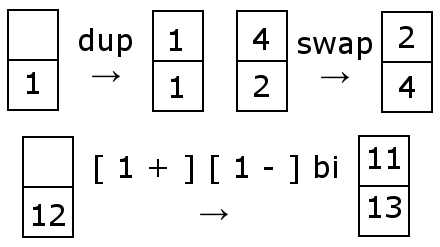
\includegraphics[height=1.1in, width=2in]{figs/stackpic}
\caption{A visual representation of a few commonly used words in 
Factor code.}\label{fig:stackpic}\end{figure}

\section{Quotations and Vocabularies}

As mentioned above, functions in Factor are idiomatically called
words. Words can be anonymously constructed from the composition
of other words. Anonymous words are called \textit{quotations} 
and are wrapped in the \texttt{[} and \texttt{]} \textit{parsing 
words} that enclose the quotation. Table~\ref{tab:parsewords}
illustrates some of the most common parsing words encountered in 
Factor code. Some words, such as \texttt{if}, take a quotation 
as an argument and use that quotation to transform the stack. 
Quotations can also be constructed using values already on the 
stack when using a pair of alternate words. For instance,
\texttt{10 '[ \_ = ]} results in the equality quotation 
\texttt{[ 10 = ]}.

Words can also be defined with formal names. New words are 
defined with a sequence of the beginning  \texttt{:} parsing word,
the given name to the word, the word's stack effect, the body of
the word, and the enclosing \texttt{;} parsing word that marks
the end of a definition. For example, consider the following 
word \texttt{product} which multiplies the contents of a sequence:

\begin{lstlisting}
: product ( seq -- p ) 1 [ * ] reduce ;
\end{lstlisting}

\noindent{}Multiple words like \texttt{product} above can be defined 
in a collection known as a \textit{vocabulary}---the Factor analog 
of a library. Vocabularies are stored within a source code file that
rests in a hierarchal subdirectory structure within the Factor 
installation directory. Each vocabulary has to explicitly reference
the vocabularies that it relies upon for operation. For example, 
a separate vocabulary that wishes to use the \texttt{product} word
above would need to include the vocabulary in which product is 
defined. Explicit declaration of necessary vocabularies allow 
Factor's compiler to ensure minimization of the compiled code. 
Compiled Factor programs only include the bare minimum code needed
for successful program execution. 

\begin{table}
  \caption{Commonly encountered parsing words.}
  \begin{tabular}{lll}
    \toprule
    \multicolumn{1}{c}{\textbf{Parsing Word}} &
    \multicolumn{1}{c}{\textbf{Semantics}} \\
    \midrule
     \verb|: ... ;|&Denotes the start and end of a named word.\\
          \verb|( ... -- ... )|&Denotes a word's stack effect.\\
	 \verb|[ ... ]|&Denotes a quotation or anonymous word.\\
     \verb|{ ... }|&Denotes an array or vector sequence.\\
     \verb|!|&Denotes a comment until end of line.\\
  \bottomrule
\end{tabular}
\label{tab:parsewords}
\end{table}

\section{Object-Oriented Implementation}
Factor is a \textit{purely} object oriented programming 
language. This means that every value used is an object. Classes
are divided into three primary types: \textit{primitive classes},
\textit{tuple classes}, and \textit{derived classes}
~\cite{pestov:Factor}. Primitive classes cannot be subclassed
and are used for primitive classes like strings, numbers, and 
words. Tuple classes are more advanced and may contain instance 
variables that, unlike generic words, are owned by the class. 
Derived classes are built from other preexisting classes and 
can take multiple forms. For example, predicate, union, and 
intersection classes can be created in the same way one might 
interpret sets from set theory. A special example is a 
\textit{mixin} class that is used often in Factor to collect 
groups of classes under a common interface~\cite{pestov:Factor}.

Another unique feature of Factor is the way in which objects
and object-specific words interact. In many object-oriented 
languages a given object has direct access to methods that are
intrinsic to that object. Factor instead uses \textit{generic 
words} that are redefined as needed to handle a given 
object-specific implementation---serving a purpose similar to 
template class functions in other languages, but with less 
restrictive implementation due to the absence of the concept 
of ownership.

\section{Factor's Development Workflow}
Programming in Factor necessitates familiarity with Factor's
interactive development environment---the \textit{Factor
Listener}. The Listener provides an interpretive playground
for the programmer to test new ideas and words on the fly without
the use of dedicated source code. When the programmer is ready
to commit to a source file, they can create a new vocabulary 
using the \texttt{scaffold} tools vocabulary and the
\texttt{scaffold-work} word. A new directory is created with an
empty source file and ready for the programmer. Once the file has
been successfully edited, the programmer can update Factor 
automatically with the new vocabulary by using either the 
\texttt{F2} key or the \texttt{refresh-all} word.

Other convenient features are provided by the Factor \textsc{ide}.
Unit tests can be defined and automatically evaluated with the
use of the \texttt{unit-test} vocabulary. Documentation files
can be created with the use of the \texttt{scaffold-docs}
vocabulary and multiple words from the auto-included \texttt{help}
vocabulary. In addition to user documentation all of the 
Factor documentation is available from within the \textsc{ide}
through the help button at the top of the interface. Word 
execution can be benchmarked at any time with the use of either 
the \verb|CTRL + T| keystroke or the use of the \texttt{time} word.
Because Factor uses an image-based compilation system, the 
\texttt{save-image} word can be used to save the state of the 
current Factor instance to a file. Images can then be loaded 
when the \textsc{ide} is launched, resulting in a faster development 
experience without the need of reloading key vocabularies for
every launch. Factor is also capable of deployment as a 
standalone executable with support for Windows,
Linux, and Mac OS, through the use of the \texttt{deploy} word.
Moreover, Factor itself also has many capable vocabularies that 
implement concepts from foreign function interfaces and \textsc{ui}
toolkits to direct \textsc{http} and \textsc{smtp} support
~\cite{pestov:Factor}.

\section{Exercises}

The following are some programming exercises that incorporate
some essential Factor concepts:

\begin{enumerate}

\item
Define a word \texttt{caesar} in a vocabulary \texttt{homework}
that takes a string of alphabetical characters and an integer 
and applies the integer to each character in the string. Your
solution must handle both positive and negative offset values.
Only include uppercase and lowercase alphabetical characters 
in the output. For example, \texttt{ABCD} with an offset of 4 
should produce \texttt{EFGH}. Factor your solution into a
primary word \texttt{caesar} and set any helper words as 
private. This problem can be solved in less than 10 lines of 
code. 

\noindent
Examples:

\begin{lstlisting}
> "SEESPOTRUN" 26 caesar .
"seespotrun"

> "SEESPOTRUN" -26 caesar .
"seespotrun"

> "ABCDEFG" 7 caesar .
"HIJKLMN"
\end{lstlisting}

% exercise 2
\item
Define a new tuple class \texttt{novel} that represents a 
fictional literary work. Include member variables that 
correspond to the novel's title, author, genre, publisher,
year of publication, and an identification number. Use 
strings for the first four variables and integers for the 
last pair. Include a constructor \texttt{<novel>} that takes
values for each variable as arguments and sets them 
automatically. Also include a word \texttt{book-print}
that takes a novel as an argument and prints the novel's
details in a simple format. 

\noindent
Examples:

\begin{lstlisting}
> "Narnia" "C. S. Lewis" "Fantasy" 
  "Geoffrey Bles" 1952 1 <novel>

--- Data stack:
T{ novel f "The Lion, the Witch, 
and the Wardrobe" "C. S. Lewis" 
"Fantasy" "Geoffrey Bles" 1950...

> book-print
Class: Novel
Title: The Lion, the Witch, and 
the Wardrobe
Author: C. S. Lewis
Genre: Fantasy
Publisher: Geoffrey Bles
Year: 1950
ID: 1
\end{lstlisting}

% exercise 3
\item
Extend the solution to problem 2 to two new classes of
books---\texttt{textbook} and \texttt{article}. For textbooks, change
the genre field to subject. For article, change the genre
field to discipline and add journal and volume fields.
Then, with the three classes, define a \texttt{mixin} class 
called \texttt{library} that will represent the union of 
different types of books. Adjust the \texttt{book-print}
word from before to be generic with templates for each type 
of book. Publish the \texttt{library} and each class in a 
\texttt{library} vocabulary.

\noindent
Examples:

\begin{lstlisting}
> USE: library
> "The C Programming Language"
  "Ritchie, D. and  Kernighan, B."
  "Computer Science" "Prentice 
  Hall" 1988 2 <textbook>

--- Data stack:
T{ textbook f "The C Programming 
Language"...

> book-print
Class: Novel
Title: The C Programming Language
Author: Ritchie, D. and Kernighan, B.
Subject: Computer Science
Publisher: Prentice Hall
Year: 1988
ID: 2

> "Factor: A Dynamic Stack-based 
  Programming Language" 
  "Pestov, S." "Computer Science" 
  "ACM SIGPLAN Notices"
  45 "ACM Press" 2010 3 <article>

--- Data stack:
T{ article f...

> book-print
Class: Novel
Title: Factor: A Dynamic Stack-based 
Programming Language
Author: Pestov, S.
Discipline: Computer Science
Journal: ACM SIGPLAN Notices
Volume: 45
Publisher: ACM Press
Year: 2010
ID: 3
\end{lstlisting}

\end{enumerate}

\section{Conclusion}
The strengths of both object-oriented and functional languages
are blended in Factor. Abstract classes, higher-order functions,
and Factor's expressive syntax give the programmer the 
flexibility needed to solve many complex problems in an elegant 
way. Factor's wide set of mature vocabularies and features allow
the programmer to focus on the greater details of a given problem.
If the curious programmer is able to overcome the learning curve 
that comes with writing concatenatively they will find a rich and 
rewarding language awaits them.  In summary, or if you will, 
in a word:

\begin{center}
\textsf{: Factor ( -{}- is ) "Object Oriented" 
"Functional Execution" +  ;}
\end{center}

\balance

\bibliographystyle{ACM-Reference-Format}
\bibliography{arnoldz3-Factor} 

\end{document}
